\begin{savequote}[75mm]
[...] to boldly go where no one has gone before [...]
\qauthor{Star Trek}
\end{savequote}

\chapter{Reinforcement learning for LARTPC detector}
\label{chap:rl-lartpc}

As this thesis centres around the intersection of particle physics and machine learning, it was quite natural to brainstorm the ideas for pushing forward this niche of science.
One of the very conclusions from studying very different applications of machine learning to many of the particle physics problems was the lack of unification.
Although many of the algorithms solve critical problems in the domain, a significant portion is highly dependent on the type of detector.

This is partially expected; after all, each of the detectors is designed for a particular branch of physics that they will study. Yet, all of those experiments study exactly the same universe and expect that the underlying rules of physics are exactly the same, and the holy-grail of particle physics, called the Standard Model aims to unify all of the branches of particle physics.

This notion is not reflected in the pursuit of machine learning algorithms for experiments.

This, and my participation in 2017 on ``Machine learning for High energy physics'' school in Oxford, pushed me to sketch an idea for a more general algorithm.

In this pursuit, I decided that although the vast sea of possible methods that stem from the supervised machine learning is ever-expanding, the nature of this branch of machine learning is too limiting.
It expects concrete examples of input-output pairs, while many of the tasks at best can only provide an estimate of the overall performance.
This is why I have chosen the Reinforcement Learning approach for further investigation.
As someone who worked both in industry and in science with artificial intelligence, I know that the fewer constraints the problem has, the harder it is to solve it. To put it mathematically, the difficulty of the problem is inversely proportional to its number of constraints. This is the cost of the generalisation.

The conceptual model for a high-level reinforcement learning definition of the general problem of both identification and tracking of the particles can be brought back to the corpuscular model of particles.
Intuitively this is how we perceive the particle, especially when considering the Feynman diagrams. In this model, a particle is an object travelling through space and being subjected to the rules of physics following decays and interactions.

Such a model can be translated into the reinforcement learning environment setting quite easily;
a particle is an agent interacting with the environment while subjected to its rules.
Just like a video game character moving through a game environment.
The agent's ability to imitate reality can be assessed by checking how well it obeys the rules of the environment.
If the agent obeys the rules, it is rewarded. If the agent does not obey the rules, it is punished (either by receiving a smaller reward, or even a negative reward).
The ideal agent/model is then the one that maximises the reward.

The rules that govern the behaviour could also be approached as a generative task, in which the goal is to produce realistic record of the behaviour of the particle.
This could be implemented as a GAN (Generative Adversarial Network) architecture, where the progress of  a generative network is assessed by comparison to the simulation rules.
But then this would mean that the task is purely about the generation of the data, and would not benefit from the conceptualisation of the physical rules in a machine learning model.
The information gained from the training could be use for particle tracking and identification, which is far more useful.
This is how we land on a reinforcement learning idea, where the data generated from the simulation is used to train a model for identification and (partially) tracking of the particle.


\section{Simulations and Data}

The inspiration for this research comes from a DeepLearnPhysics public dataset.
That dataset contains simulation data, which includes pairs X and Y of both the simulations of records of particles in the LARTPC and their ground truth classification in each position in space.
The environment for the reinforcement learning was prepared using that simulation data..
Although the code details of the simulation weren't explicitly mentioned for the dataset used in this study, the DeepLearnPhysics collaboration prepared a preprint article for the new version of the open dataset \cite{adams2020pilarnet}, in which they mention that the simulation was prepared using LARTSOFT\cite{Snider:2017wjd} and GEANT4\cite{ALLISON2016186}.

The simulation generates particles inside a LARTPC detector \cite{dlp_tutorial}, and their progress in time is recorded by the detector.
The source point of the generated particles is uniformly distributed in 3D.
The total particle multiplicity is set to be uniform between 2 to 5.
There is an equal and uniform probability of generating any particle from four categories presented in table:


\begin{table}[h]
\begin{center}
\begin{tabular}{ |c|c|c|c|}
\hline
Category & Particle Type & Energy range (uniform) & Multiplicity  \\
\hline
0 & light lepton (electron or muon) & 50 to 1000 $MeV$ & 0 to 3  \\
1 & gamma ray & 50 to 1000 $MeV$ & 0 to 2  \\
2 & charged pion (pion or anti-pion) & 50 to 1000 $MeV$ & 0 to 2  \\
3 & proton & 50 to 400 $MeV$ & 0 to 3  \\
\hline
\end{tabular}
\caption{\label{tab:sim_probs} Table of simulated particle properties for LARTPC data generation.}
\end{center}
\end{table}

The energy deposition for an individual particle is stored in a 3D voxel of 0.5 $cm^{3}$ in $MeV$ units, but later it is saved with a scaling factor of 100 \cite{dlp_tutorial}.
Next, the 3D data is projected onto three 2D planes.
Then the data that contains less than 5 pixels in any given projection with a pixel value lower than 0.1 MeV is rejected.
The values of voxels lower than 0.1 Mev are trimmed to 0.
For the purpose of this research I do not use full 3D voxelised information, but one of the 2D projections.


\section{Dataset}

The dataset generated from the simulations and used in this research is available at the DeepLearnPhysics collaboration website \cite{dlp_website}.
This dataset contains 15.000 training samples as well as 10.000 test samples.
Each of the samples contains a single simulation of a signal event, as discussed in the previous subsection.
The simulations are saved as two 2D images - a source image where only information is the energy deposit in the pixel and a target image - where pixels hold the information about the type of the particle in the given pixel.
The target image contains 3 types of pixels: background, EM-shower particles, and track particles (i.e. not EM-shower).

As the images are genreated from a simulation, they can have arbitraly large size.
This is also reflected in the RL environment mentioned later in the chapter.
For the examplary solution the 256x256 in size of the image is used.


\begin{figure}[H]
\centering
\begin{subfigure}[b]{\textwidth}
\centering
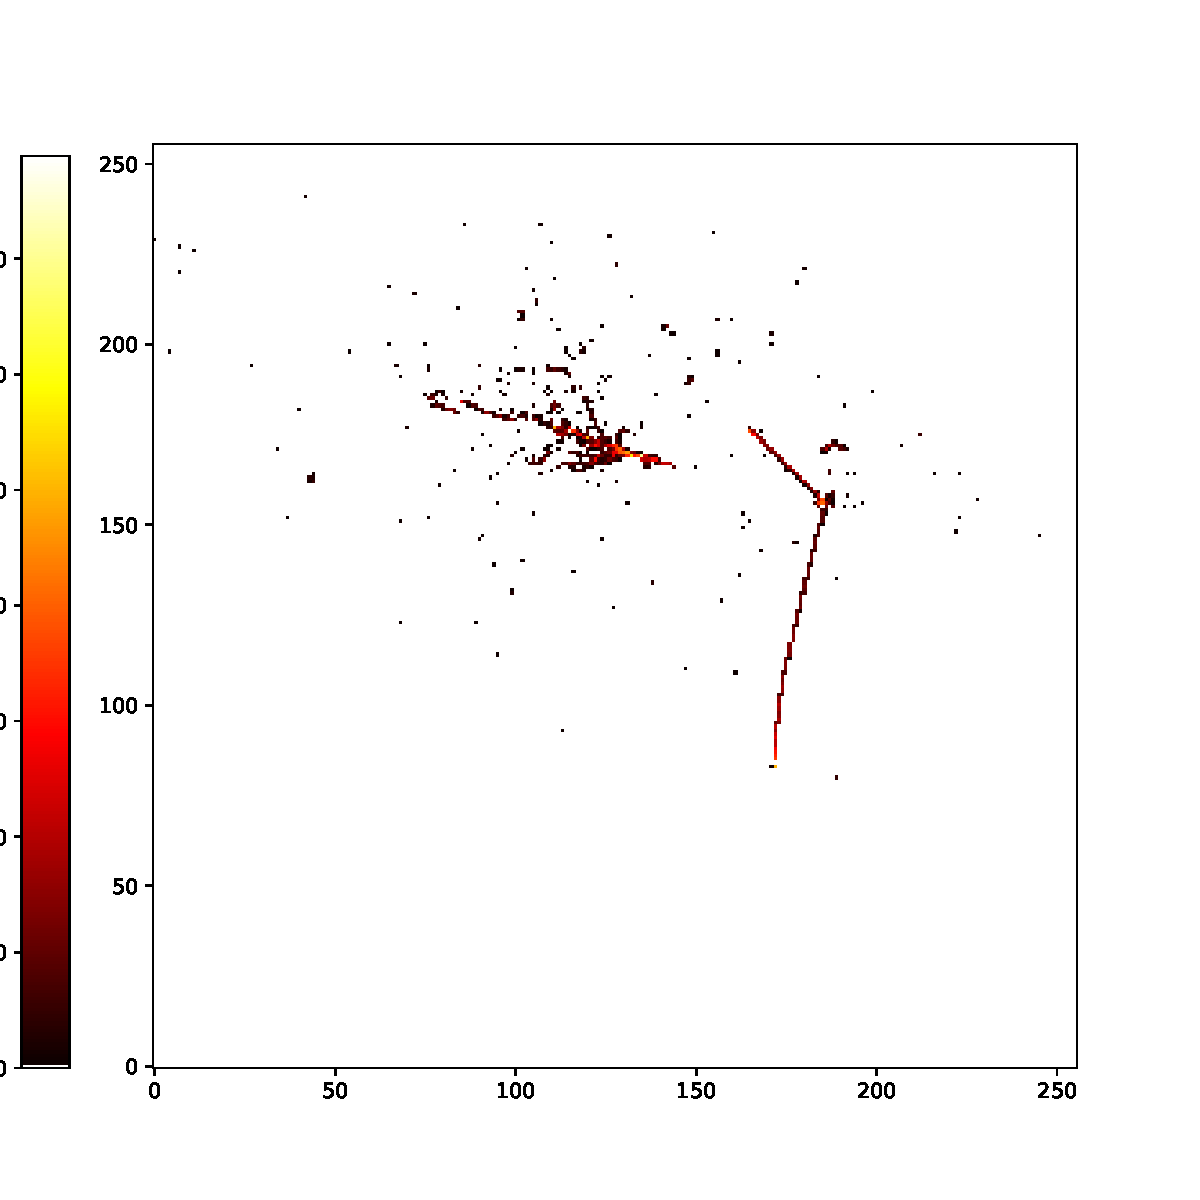
\includegraphics[width=0.7\textwidth]{figures/chapter7/examplary_data_x.pdf}
  \end{subfigure}

\begin{subfigure}[b]{\textwidth}
\centering
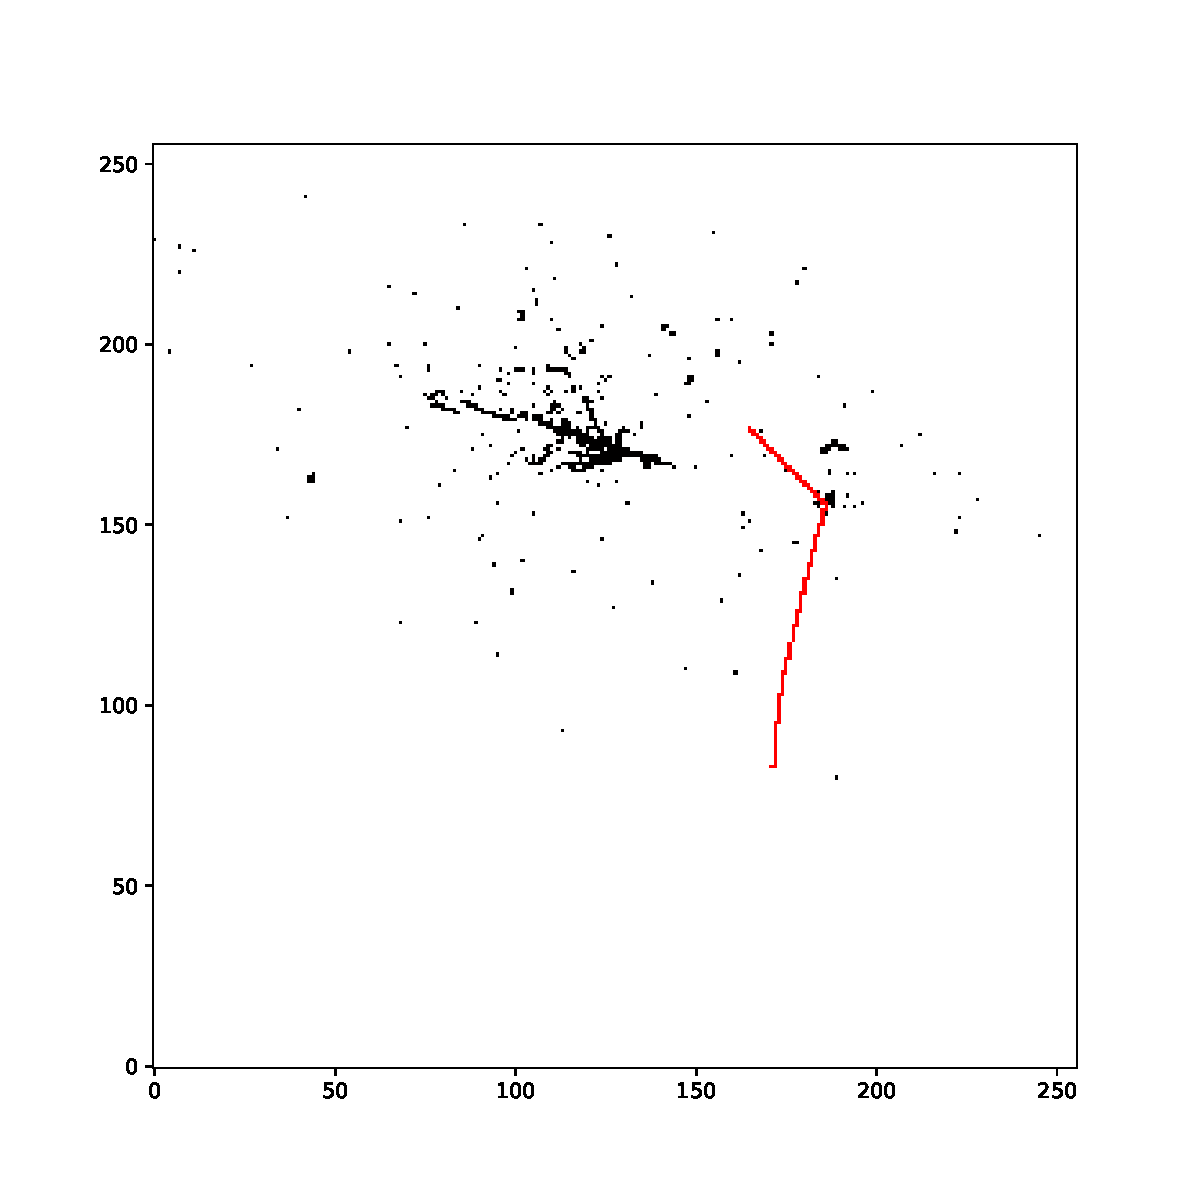
\includegraphics[width=0.7\textwidth]{figures/chapter7/examplary_data_y.pdf}
  \end{subfigure}
\caption{Exemplary data from the LARTPC dataset. \textbf{Top} image is the source input, and the \textbf{bottom} image is the desired output (target)}
\label{fig:lartpc-data-example}
\end{figure}

\begin{figure}[H]
\centering
\begin{subfigure}[b]{0.67\textwidth}
    \centering
    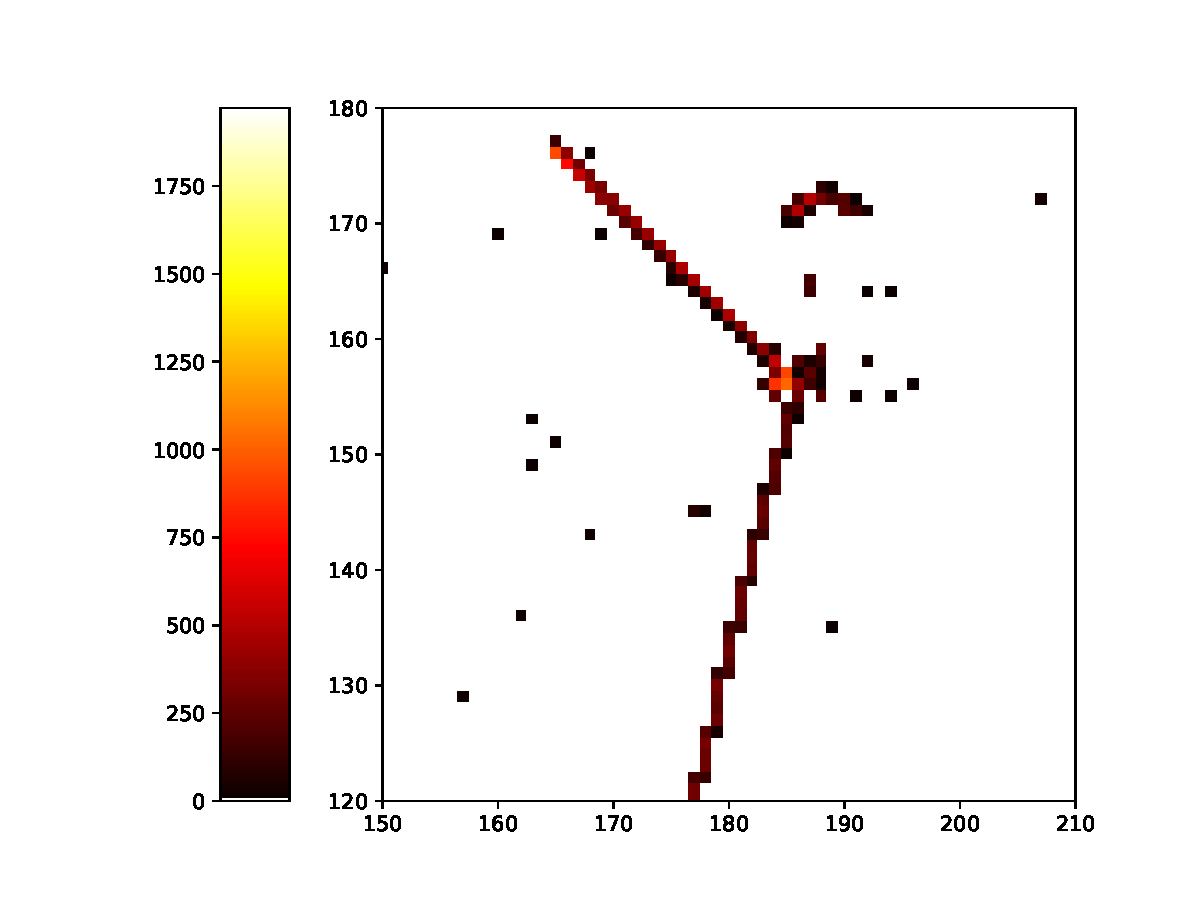
\includegraphics[width=\linewidth]{figures/chapter7/examplary_data_zoom_source.pdf}
\caption{Source (X)}
   \label{plot:lartpc-example-source-zoom}
  \end{subfigure}
\begin{subfigure}[b]{0.67\textwidth}
    \centering
    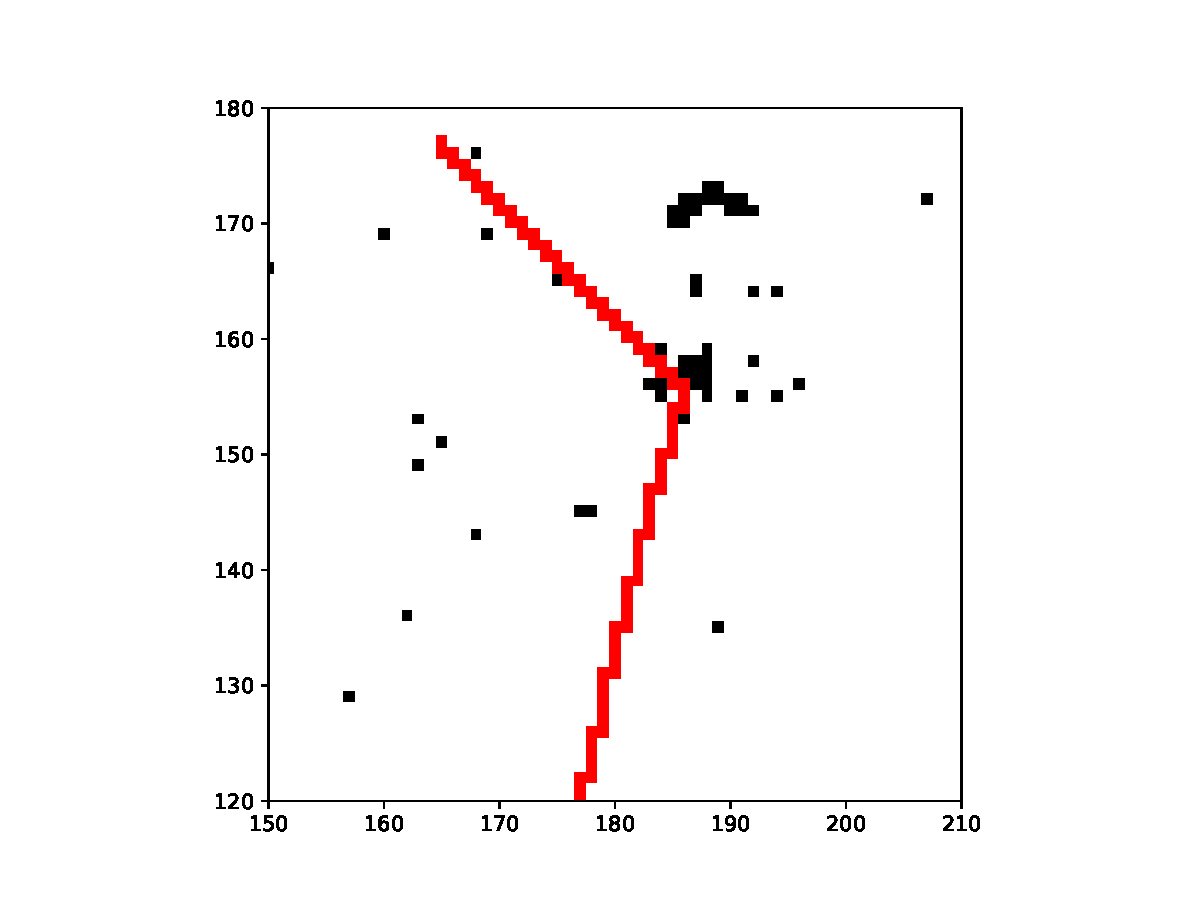
\includegraphics[width=\linewidth]{figures/chapter7/examplary_data_zoom_target.pdf}
\caption{Target (Y)}
    \label{plot:lartpc-example-target-zoom}
  \end{subfigure}
  \caption[Examples of zoom]{Examplary data zoomed into a smaller region.}

    \label{plot:lartpc-example-zoom}
\end{figure}



% \begin{figure}
%     \centering
%     \begin{subfigure}[b]{0.5\textwidth}
%     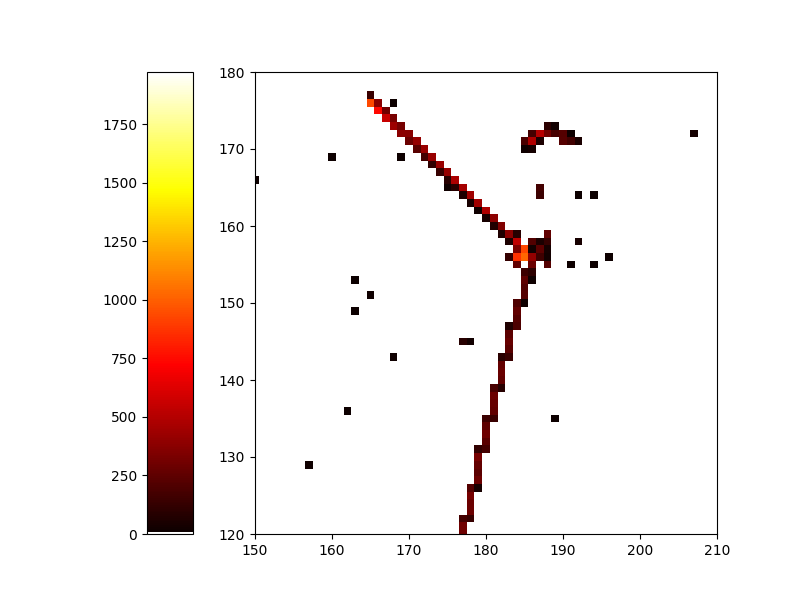
\includegraphics[width=\linewidth]{figures/chapter7/examplary_data_zoom_source.png}
%     \caption{ .}
%    \label{plot:lartpc-example-source-zoom}
%   \end{subfigure}

%   \begin{subfigure}[b]{0.5\textwidth}
%     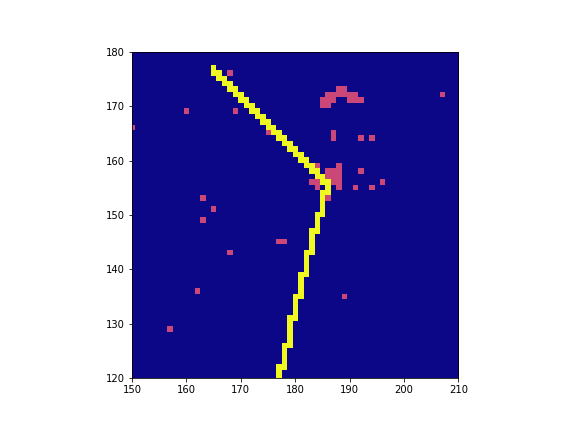
\includegraphics[width=\linewidth]{figures/chapter7/examplary_data_zoom_target.png}
%     \caption{ .}
%    \label{plot:lartpc-example-source-zoom}
%     \label{plot:lartpc-example-target-zoom}
%   \end{subfigure}
%       \caption[Examples of zoom] Examplary data zoomed into a smaller region.}
%    \label{plot:lartpc-example-source-zoom}
%     \label{plot:lartpc-example-target-zoom}
%     \label{plot:lartpc-example-zoom}

  % \end{figure}


%% data http://deeplearnphysics.org/DataChallenge/
%% generation http://deeplearnphysics.org/Blog/2018-01-01-BrowsingSegmentationData_v0.1.0.html#overview
%% https://github.com/DeepLearnPhysics/LArTPCEventGenerator



\section{Environment}

The reinforcement learning approach requires a ``game-fication'' of the problem.
That means that we essentially want to turn the problem into a game, preferably one that allows for gaining points along with the progress of playing.
For this purpose the gym-lartpc environment was created \cite{gymlartpc}.
It is based on the openai-gym library \cite{openaigym}.
As explained in the Sec. \ref{sec:deep_rl} game should consist of an environment and an agent.
The agent can interact with the environment and modify it.
In the case of lartpc data, the agent will be an analogue to a particle, and the environment is analogue to the space inside LARTPC medium.
Before the detail of implementation itself are presented, it is vital to present a formalisation of the problem.

\subsection{Formalisation}

The usual framework for mathematical formulation of the reinforcement learning problem requires a definition of the problem in terms of Markov Decision Process (see Sec. \ref{sec:rl_mdp}) or MDP.
This subsection will present steps towards representing the gym-lartpc environment as an MDP, along with introducing key objects that comprise the lartpc-gym package.

\subsubsection{Maps}

In the sense of translating the LARTPC data into game, the images of the dataset can be thought of as maps, which the agent will explore.
Although original dataset samples contains source and target, for the purpose of creating the game environment an additional map called canvas is added.
The agent will explore the source map ($S$, 256x256) and by using it the agent will try to approximate the target map ($T$, 256x256). An example of source and target can be seen at \ref{fig:lartpc-data-example}.
The output of the approximation is saved on the canvas map ($C$, 256x256x3 - the last dimention is one of the thre categories), which is the actual output of the algorithm.
The canvas map $C$ is used to create an image containing categorised pixels. 
This image then can be compared with the target of a given sample.
The majority of the environment states are not available for the agent, so only its nearest neighbourhood is considered.
This neighbourhood can be expressed as a quadratic window n x n.
In total there are three types of window objects source map window $W^{S}$, canvas map window $W^{C}$ and target map window $W^{T}$.

It is useful to mentally imagine this task and the usage of those three maps as learning to paint a picture, using a sketch.
The source map $S$, can be thought of as an sketch of a ready painting $T$. Then, the task is to paint a picture $C$ which will be the most resemblant the $T$, using only $S$ as reference.

\subsubsection{States}


It is assumed that the agent occupies a position on the map $p\_x,p\_y$, with each step, this position may change.
There is only a small subset of states from an environment available for the agent, defined by the window on the map.
The center of the window is always position at the agent position $p\_x,p\_$
The state in the current timestep $t$ can be denoted as $s_{t}=(W^{S}_{t}, W^{C}_{t})$. These states create state space $S$ of MDP.

\subsubsection{Actions}
\label{sec:rl_action}

In such defined environment the total action can be expressed as composed of two sub-actions:

\begin{description}
\item[Movement action] - a decision on the direction of the next step in the game, expressed as a 2D vector $m_{t}$, where $[1,1]$ is a movement by one pixel right (x-axis) and one pixel up (y-axis).

\item[Put action] - a KxKx3 tensor denoted by $c_{t}$. This matrix will be pasted into the canvas map C, using proper window size on the coordinates defined by the center $p\_x,p\_$.
The the last dimension of the tensor denote probability of given pixel belonging to one of the three categories (background, EM-shower particles, and track particles).
The centre coordinate of the $c_{t}$ has the same coordinates as the Source Window centre.


\end{description}

The action can be expressed as a tuple $a_{t} = (m_{t}, c_{t})$.
Going back to analogy of painting the picture, one can imagine, that the $m_{t}$ would be direction of a stroke, and $c_{t}$ would be set of colors to use to paint. 
The actions create action space $A$ of MDP.

\subsubsection{Rewards}

Finding a correct reward function in reinforcement learning is a challenge.
Therefore, this part is open for interpretation by the user in the implementation of the environment.
That being said, the default implementation for the reward $R_{t}$ calculation follows the algorithm:

\begin{align}
& R_{1} = N_{discovered}(W^{c}) \\
& R_{2}= N_{\mathrm{nonzero}}(W^{s}) + 0.9 \times R_{1}\\
& R_{3} =
\begin{cases}
    R_{2}-5,& \text{if } R_{2}== 0\\
    R_{2},              & \text{otherwise}
\end{cases} \\
& R =
\begin{cases}
    R_{3}-15,& \text{if } Center(W^{s}) == 0\\
    R_{3},              & \text{otherwise}
\end{cases}
\label{eq:reward}
\end{align}

Where \(N_{discovered}(W^{c})\) is the number of the pixels in $W^{c}$ which haven't been categorised (painted) yet.
This encourages to find the pixels that haven't been visited yet.
The term $N_{\mathrm{nonzero}}(W^{s})$ is the number of non-zero (empty) pixels in source window $W^s$.
The term $R3$ is a punishment when both $R1$ and $R2$ are zero, meaning that the source window is empty, and target window is already fully processed.
Finally, $R$ adds a punishement if the central position of the source window is empty.

In summary, this reward system encourages exploration of both non-empty pixels on source map, and non-processed pixels using canvas map.
The reward highly discourages to stay in one place, or in locations in which the source map has zero valued pixels.
% The goal of this reward is to encourage the exploration of non-empty pixels by the agent. The $R_1$ term rewards exploration of areas where the $\mu^{c}$ is empty. The $R_2$ modifies the $R_1$ by rewarding exploration of $\mu^{s}$. The $R_3$ penalises no exploration, and the last equation also penalises the model for stepping into the background.

\subsection{MDP and POMDP}
% https://www.quora.com/Why-can-deep-reinforcement-learning-be-combined-with-recurrent-neural-networks-and-LSTMs-Does-this-violate-the-Markov-property-the-basis-of-reinforcement-learning
% file:///home/mwm/Downloads/make-03-00029.pdf
% https://cdn.openai.com/dota-2.pdf
% https://arxiv.org/pdf/1507.06527.pdf

The elements of states, actions and rewards, along with the logic of the lartpc-gym environment, give rise to a Markov Decision Process Formulation (see Sec \ref{sec:rl_mdp}), and allows us to use standard reinforcement learning methods to solve the problem posed by the environment.

But careful readers can notice that the term $R_{1}$ may be breaking the Markov property.
Indeed, depending on the defined reward function, the environment can break the Markov property. 
And with the reward defined as in Eq. \ref{eq:reward} it does brake the Markov property, because the new state with the canvas map is constantly updated by the agent, canvas window $W^{c}_{t}$ contains the result of put action $c_{t-1}$ from the previous step. It is important to note that in this case, only the number of already visited locations on the map, that are apparent in the $W^{c}_{t}$ is contributing to the reward, and not the values contained on $W^{c}_{t}$.

Yet, the breaking of the Markov property does not mean that the environment is unsolvable with reinforcement learning.
Many of the novel and state of the art solution to gaming environments, such as AlphaStar \cite{Vinyals2019}, or OpenAI five \cite{doi.org/10.48550/arxiv.1912.06680} are known to be rather non-markovian.
In this case, another formulation of the problem may be useful: POMPD (Partially Observable MDP).
POMDP can be expressed as 6-tuple $(S,A,P,R,\Omega,O)$ , where $(S,A,P,R)$ are the same as in MDP, but now the agent doesn't observe the states directly, but rather through observation $o \in O$.
This observation is sampled according to some distribution $o \sim O(s)$. The $O(s)$ is a function that provides an observation given the state $s$ with some probability.
In essence what that means is that the full underlying state of the environment may be obscured by the $O$.
In a case of non-markovian environments the state can be understood as state with it's past history, and the observation $O$ provides only the most recent state, obscuring the past.
A classical Deep Q-Learning has no explicit mechanism to solve the problem stated in this way, but some works \cite{doi.org/10.48550/arxiv.1507.06527} show that by adding the recurrency to the network, this becomes solvable.
In the case of the model presented here, there is a hidden recurrent dependency of the model, as it reads and writes values to the target canvas.

\section{Gym-lartpc package}
The environment formulated in the previous section was implemented in a Python Package called ``gym-lartpc'' \cite{gymlartpc}, which contains openai-gym interface.
Openai-gym \cite{openaigym}is a popular open-source project containing reinforcement learning environments.
Each of the environments provides exactly the same style of the interface.
The minimal requirement for creating compatible environment with openai-gym is to extend the \textbf{gym.Env} class, and provide \textbf{step(action)}, \textbf{reset()} and \textbf{render()} methods.

%%Although the package interface to the openai-gym environment contains its own classes separate from the openai-gym, which combine into the implementation of the game.

Although the package has the openai-gym environment interface, it also provides a separate custom interface for more sophisticated options for users' convenience.

Although the gym-lartpc package does not contain official API documentation, the code itself is very clean and reads well enough.

\subsection{Classes}

The most important classes in the package are LartpcData, DetectorMaps, Lartpc2D, and Cursor.


\begin{description}
\item[Cursor] denotes a region on any map (Source, Canvas, Target). Its x and y coordinates and can be used to get or set a window of values on a map.

\item[DetectorMaps] contains Source Canvas and Target maps together. It allows getting random positions on maps and nonzero positions.

\item[Lartpc2D] contains the logic of the game. Holds both Cursor instance and DetectorMaps instance.
It's \textbf{start()} method allows to start a new game. \textbf{step(action)} can be used to make a step in the game environment.

\item[LartpcData] uses either a path to a folder containing the data in the ``.npz'' format or a list of files that contain training data. It can be used to get a tuple of source and target maps as a python generator object.

\end{description}

\subsection{Example game}

\begin{listing}[!ht]
\begin{minted}{python}
def bot_replay(data_path, viz=True):
    max_step_number = 20
    data_generator = data.LartpcData.from_path(data_path)
    result_dimensions = 3
    game = Lartpc2D(result_dimensions, max_step_number=max_step_number)
    vis = Visualisation(game)
    agent = BotAgent(
        game
    )
    for iterate_maps in range(30):
        map_number = np.random.randint(0, len(data_generator))
        game.detector.set_maps(*data_generator[map_number])
        for iterate_tries in range(10):
            game.start()
            for model_run_iteration in range(game.max_step_number):
                current_observation = game.get_observation()
                action = agent.create_action(current_observation)
                state = game.step(action)
                vis.update(0)
                if state.done:
                    break
\end{minted}
\caption{Example of usage of Lartpc2D class. This function implements visualisation with a random agent.}
\label{listing:rl_example}
\end{listing}

\begin{sloppypar}
The listing in \ref{listing:rl_example} shows an exemplary use of the Gym-lartpc package.
The Lartpc2D class accepts a dimension of the result and a maximum number of steps as arguments.
Here the result dimension means the size of the two-dimensional window that will be used on the output map.
When using the \textbf{game.detector.set\_maps()} method the maps are set to a random source target pair coming from LartpcData class.
The \textbf{game.start()} resets the state of the environment and assigns a random, non-zero, non-visited location to the cursor in the environment.
Then, the current observation of the game can be accessed by the \textbf{game.get\_observation()} attribute and action can be passed using \textbf{game.step()} method. This will move the cursor according to the movement contained inside the action and will change the value on the canvas map at the scope occupied by the cursor.
It is worth noting that three types of objects are exchanged between the environment and agent (see corresponding listing in \ref{listing:rl_observables});
\end{sloppypar}

\begin{description}
\item[Action2Dai] which embodies an action $a_{t} = (m_{t}, c_{t})$. Contains \textbf{movement\_vector} attribute ($m_t$), which is eected to be a numpy array of shape 1x2 (a vector of length two), and a \textbf{put\_data} ($c_t$) which is expected to be 2D array of a shape compatible with result dimension. This is the action described in Sec. \ref{sec:rl_action}.

\item[State2Dai] which contains the state of the game, as expected by the openai-gym. The state of the game in the gym-lartpc is a tuple consisting of current observation of the environment, reward, ``done'' flag, and empty string.
The empty string is a space-holder for any additional information coming from the environment required by the openai-gym implementation. ``Done'' flag is true if the game has ended.
This condition may occur if the agent has exceeded the allowed number of moves, or cannot make the action (steps outside the map).
The reward is the float value as described in the previous section.

\item[Observation2Dai] consists of three windows in a given position $W^{S}$ $W^{C}$ $W^{T}$.
\end{description}

The main loop of the game works in the following way:

\begin{enumerate}
    \item The observation of the game is made using the \textbf{game.get\_observation()}.
  \item The agent uses the observation with \textbf{agent.create\_action(observation)} method, and creates an instance of \textbf{Action2Dai} object containing the action to take in the next step.
  \item The game environment processes the action using \textbf{game.step(action)}. First, it applies the change specified in the classification, then it changes internally the position of the cursor, and returns a new state of the game.
\end{enumerate}


\begin{listing}[!ht]
\begin{minted}{python}
@dataclass
class Observation2Dai(StaticTyped):
    source: NDArray[(typing.Any, typing.Any), np.float32]
    result: NDArray[(typing.Any, typing.Any, 3), np.float32]
    target: NDArray[(typing.Any, typing.Any), np.int32]

@dataclass
class State2Dai(StaticTyped):
    obs: Observation2Dai
    reward: float
    done: bool
    info: object

@dataclass
class Action2Dai(StaticTyped):
    movement_vector: NDArray[(1,2), np.int64]
    put_data: NDArray[(typing.Any, typing.Any, 3), np.float32]
\end{minted}
\caption{Impelemntation of \textbf{Observation2Dai}, \textbf{State2Dai}, \textbf{Action2Dai}.}
\label{listing:rl_observables}
\end{listing}

\subsection{Visualisation}

The package also allows for visualisation of the game, implemented using PyQt.
This feature allows for step by step basis watching of the progress of the algorithm, using the space key.
The Fig. \ref{fig:lartpc-visual} contains a screenshot of the visualisation running in 6 different windows.
The top row of windows depicts the the parts of the maps visible to the the agent, and the lower row of windows shows the position of the agent on each of the maps.

\begin{figure}[H]
\centering
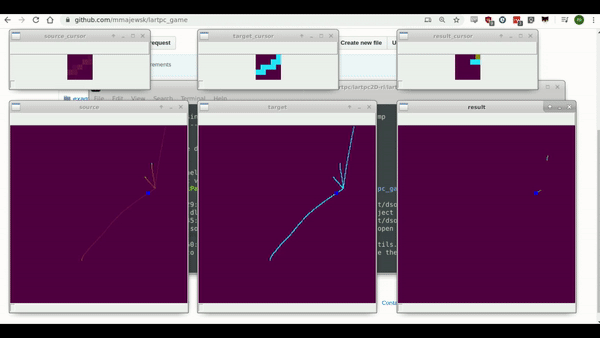
\includegraphics[width=\textwidth]{figures/chapter7/lartpc_visual.png}
\caption{Visualisation in the gym-lartpc package.}
\label{fig:lartpc-visual}
\end{figure}

\section{Deep Q-learning solution}
\begin{figure}
\begin{subfigure}{.45\textwidth}
  \centering
  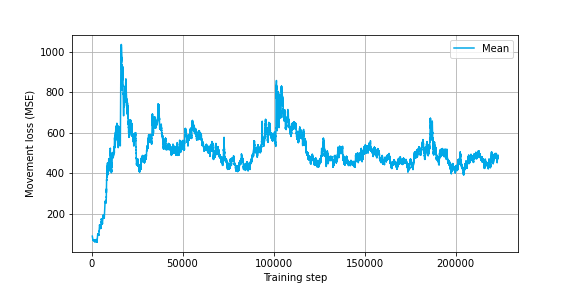
\includegraphics[width=1.2\linewidth]{figures/chapter7/loss.png}
  \caption{Mean square error loss}
  \label{fig:rl_loss}
\end{subfigure}%
\hspace{1em}%
\begin{subfigure}{.45\textwidth}
  \centering
  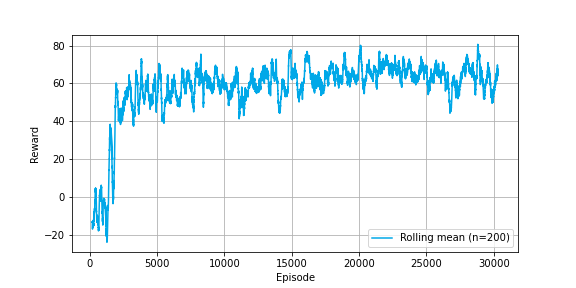
\includegraphics[width=1.2\linewidth]{figures/chapter7/reward.png}
  \caption{Reward curve}
  \label{fig:rl_reward}
\end{subfigure}
\caption{The learning process of the baseline DDQN.  }
\label{fig:rl_learning}
\end{figure}

\begin{sidewaysfigure}[ht]
  \centering
  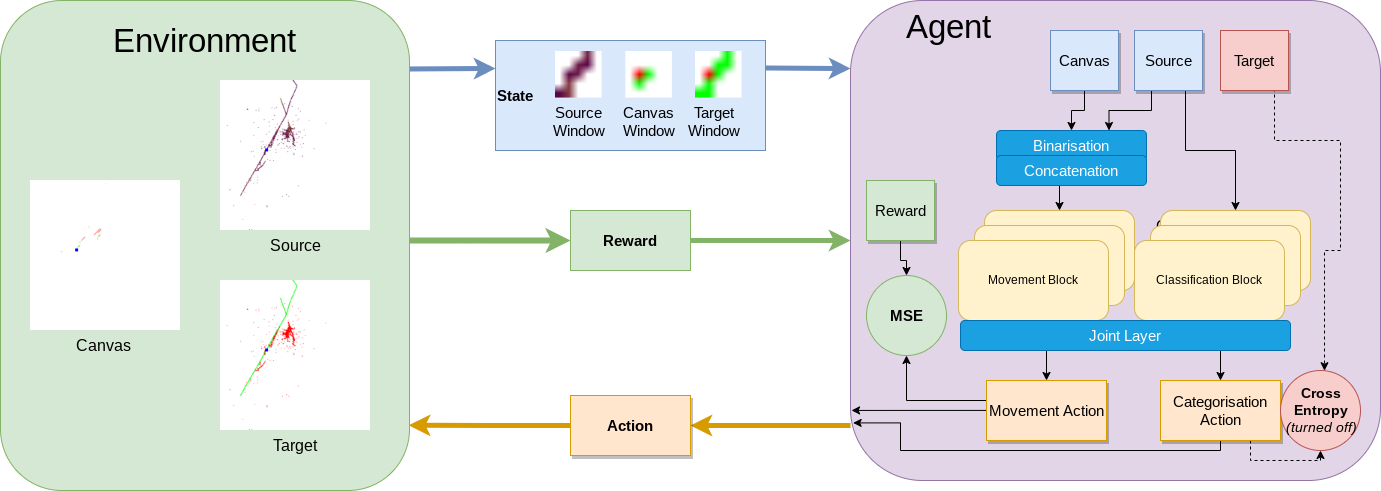
\includegraphics[width=\textwidth]{figures/chapter7/lartpc_rl_flow.png}
  \caption{Reinforcement learning setting for learning the DDQN algorithm.}
  \label{fig:settings}
\end{sidewaysfigure}

With all of the accompanying code of the lartpc game, it is much easier to brainstorm possible solutions.
There is a vast range of reinforcement learning algorithms. Probably the two most popular approaches are those based on DQN (Sec. \ref{sec:dqn}) and policy gradients \footnote{
Policy gradient methods in contrast to DQN (or value based methods), do not seek a best action, given states, but learn the probabilistic mapping of from state to value}.
The most successful solution to the problem posed by the environment in our research was DDQN, with Memory Buffer.

The Fig. \ref{fig:settings} presents interaction of the agent and the environment.
The environment, containing three maps, outputs an observation state, consisting of three smaller windows, and after each action provides the reward.
The agent uses the \textit{canvas} and \textit{source} information in two blocks, called movement block and classification block.
The higher level conceptualisation of the input and output to the agent can be seen in Fig. \ref{fig:rl_inp_out}.
The movement block is responsible for selecting the direction in which to move in upcoming action (Movement Decision).
The classification block chooses the values that it should update the canvas window with (Canvas Output Window).
Additionally, both blocks outputs undergo the operation of concatenation and are fed to a unifying block, which allows for the mixing of the information, and then creates appropriate outputs.

The classification block was pre-trained using a random sampling of the dataset images, with an appropriate window used as an output. It was pre-trained to the level of $86\%$ of accuracy. The hyper-parameters of the network can be seen in Tab. \ref{tab:rl_conv_params}.

The Fig. \ref{fig:rl_net} presents the final version of the agent neural network.
The Canvas window input, and source input are both binarised and concatenated together.
Then they are presented as input to the movement block, which consists of 5 fully connected layers intertwined with ReLU activation function.
The Source input is also presented as an input to the classification block.
The classification block consists of smaller blocks of fully connected layer, batch normalisation, ReLU, and dropout.
These blocks of four layers are repeated four times, ending with a fully connected layer that scales the output.
Output from both blocks is concatenated and passed to three fully connected layers, the output of which is divided into Movement output and Classification output.

\begin{figure}[ht]
  \centering
  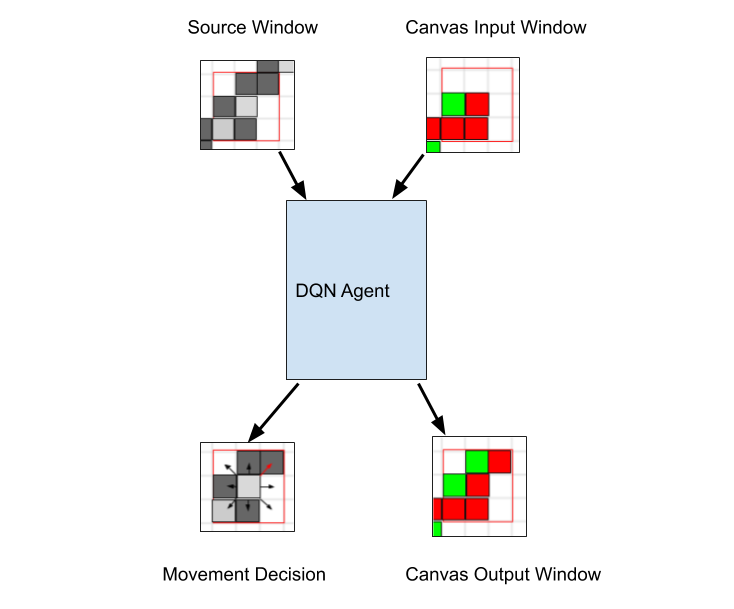
\includegraphics[width=0.8\linewidth]{figures/chapter7/network_output_input.png}
  \caption{Exemplary input and output states for the neural network used in the analysis. The network receives both Source and Canvas input windows, and outputs a movement and put actions.}
  \label{fig:rl_inp_out}
\end{figure}


\begin{figure}[ht]
  \centering
  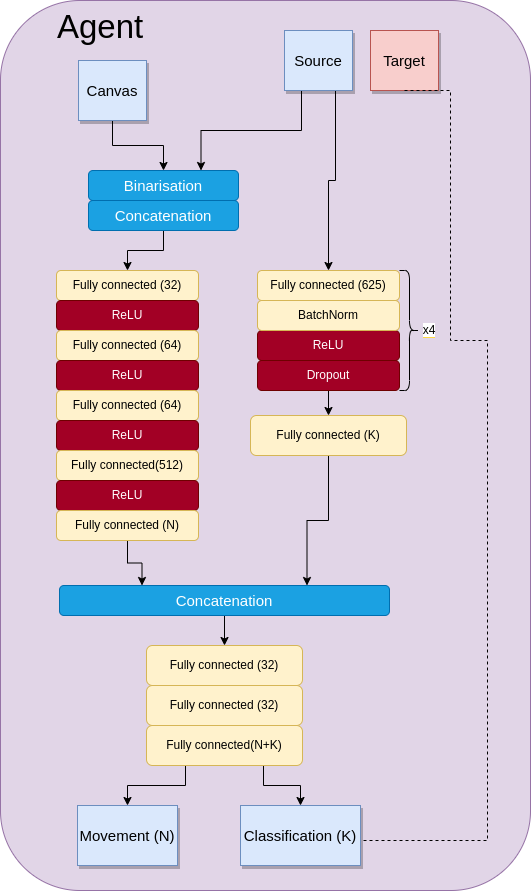
\includegraphics[width=0.8\textwidth]{figures/chapter7/lartpc_rl_network.drawio.png}
  \caption{The complete model of the employed agent neural network. Source and Canvas input windows enter the movement block after binarisation and concatenation. The Source input alone also enters the classification block as is. The movement block returns a vector of size N. N is the number of possible movement directions (usually N=8 - any neighbouring pixel). The classification block returns a vectorised matrix of classified pixels, of length K. Usually K=1 or K=9. Both blocks outputs are then concatenated and passed to the joint layer, which outputs a vector of size N+K.}
  \label{fig:rl_net}
\end{figure}

% https://app.neptune.ai/mmajewsk/fresh-lartpc/e/FRES-82/source-code?path=source_code&file=main.py&attribute=files&filePath=.
\begin{table}[h]
\begin{center}
\begin{tabular}{ |c|c|}
\hline
Parameter & Value\\
\hline
batch\_size & 128  \\
droput\_rate & 0 \\
input\_window\_size & 5\\
outpu\_window\_size & 1\\
result\_outpu & 3\\
\hline
\end{tabular}
% https://app.neptune.ai/mmajewsk/lartpc-conv/e/LAR1-9/all?path=parameters
\caption{\label{tab:rl_conv_params} The parameters used for training the convolutional neural network for simple classificiation}
\end{center}
\end{table}

\subsection{Learning}


\begin{table}[h]
\begin{center}
\begin{tabular}{ |c|c|}
\hline
Parameter & Value\\
\hline
gamma & 0.99 \\
batch\_size & 32 \\
reaplay\_size & 10 000 \\
learning\_rate & 1e-4\\
epsilon\_start & 3\\
epsilon\_final & 0.01 \\
max\_step\_number & 8 \\
trials & 8 \\

\hline
\end{tabular}
% https://app.neptune.ai/mmajewsk/lartpc-conv/e/LAR1-9/all?path=parameters
\caption{\label{tab:rl_params} The parameters used for training the convolutional neural network for simple classificiation}
\end{center}
\end{table}
The details of the training process are out of the scope of this description and may be found in the github repository \cite{dqn_lartpc}.
The table \ref{tab:rl_params} shows some of the parameters used for the training of the DQN model.
From the training quality metrics, depicted in the Figure \ref{fig:rl_learning}, one can see that the value of the reward function is growing, which proves that the model is maximising the reward. You can also see that the MSE loss function grows and then drops. This is attributted to a high epsilon value at the start and the memory buffer being filled with more uncomplicated episodes. Then the complexity of the task grows when the agent learns to explore, and then overall slowly decreases and stabilises as it learns.
It is by no means trivial to evaluate the performance of a reinforcement learning agent by only basing it upon the loss metrics and rewards defined in the previous section. The difficulty of the problem may fluctuate, as some parts of the images are easier to solve than others, the actions of the agent may influence future difficulty, and the epsilon-greedy \footnote{epsilon-greedy algorithm chooses either an action generated by the model, or completely random action based on a $\epsilon$ probability} actions introduce randomness into the process. The evaluation by observation of the agent behaviour was necessary.
It is observed that the agent indeed was following the tracks of the particles, but in the case of a more significant number of possible steps, the agent tended to ``escape'' an area with only an isolated non-zero pixel visible.

\section{Results}
The proposed DDQN solution to the problem posed by the gym-lartpc environment is meant to serve as a baseline for future research. DDQN has proved to be capable of performing very basic navigation through the decay tree. The goal of this baseline study is to show how the gym-lartpc environment can be used.
I invite other researchers to use our environment for future experimentation with reinforcement learning, which is openly available in the GitHub repositories\cite{gymlartpc} \cite{dqn_lartpc}.
The future course for this work may include removing canvas as the feedback input and using a recurrent layer in the network.
The other exciting possible extension could be rewarding the model to predict the direction and classification not for the current step but rather for the next step. This prediction could be applied to the environment and then fed back as an input to the model, generating new predictions and forming a feedback loop.
Suppose one would translate the data read from any other experiment to the same voxel representation and scaled similar energy deposits (maintaining the same domain of particles). In that case, it might be possible to reuse the same model, or expand the simulation data, to create a single model for different detectors.

The presented environment is the main focus of this study, and has the potential to be the groundwork for a more unified machine-learning-based model of physics coming from high energy physics experiments.
A cross-experimental framework could shift a focus from researching particular branches of physics (neutrino physics, b-hadron physics, particle showers, etc.) to more holistic research that accounts for all of the effects met in these particular areas.
A model suitable for multiple experiments could help us better understand the link between the parts of physics studied by those experiments.
I believe that the reinforcement learning-based model also has the potential to be used for creating simulations, as it may be computationally less expensive.

%%% Local Variables:
%%% mode: latex
%%% TeX-engine: xetex
%%% TeX-command-extra-options: "-shell-escape"
%%% TeX-master: "../dissertation"
%%% End:
